\chapter{Data Transfer}\label{chap:data-transfer}

\section{Introduction}

In this chapter, an algorithm for conservative data transfer between curved
meshes will be described. This has practical applications to many methods in
computational physics. Data transfer is needed when a solution (approximated
by a discrete field) is known a \textbf{source} mesh and must be transferred
to a \textbf{target} mesh. In many applications, the field must be conserved
for physical reasons, e.g. mass or energy cannot leave or enter the system,
hence the focus on \textbf{conservative} data transfer. A few
scenarios where data transfer is necessary will be considered below to
motivate the ``black box'' data transfer algorithm.

Since data transfer is so commonly needed in physical applications, this
problem of conservative interpolation has been considered already for
straight sided meshes. The \textbf{common refinement} approach in
\cite{Jiao2004} is used to compare several methods for data transfer across two
meshes. However, the problem of constructing such a common refinement is
not discussed. The problem of constructing such a refinement is considered
in \cite{Farrell2009, Farrell2011} (called a supermesh by the authors).
However, the data transfer becomes considerably more challenging for curved
meshes. For a sense of the difference between the straight sided and curved
cases, consider the problem of intersecting an element from the source mesh
with an element from the target mesh. If the elements are triangles, the
intersection is either a convex polygon or has measure zero. If the elements
are curved, the intersection can be non-convex and can even split into
multiple disjoint regions.

\subsection{Lagrangian Methods}

\begin{figure}
  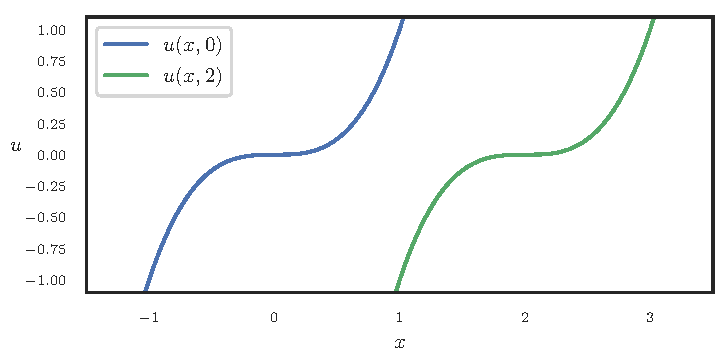
\includegraphics{../images/curved-mesh/simple_transport.pdf}
  \centering
  \captionsetup{width=.75\linewidth}
  \caption{The solution to \(u_t + u_x = 0, \; u(x, 0) = x^3\) plotted in
    the \(xu\)-plane. Demonstrates simple transport of
    the solution.}
  \label{fig:simple-transport}
\end{figure}

The method of characteristics helps transform partial differential equations
into ordinary differential equations by dividing the physical domain into
a family of curves. For example, the simple transport equation
\begin{equation}\label{eq:simple-transport}
u_t + c u_x = 0
\end{equation}
can be transformed when restricting to the family of lines
\(x(t) = x_0 + c t\). On these lines \(u(x(t), t)\) is constant, by
construction, and so the solution is ``transported'' from \(u(x_0, 0)\)
along each characteristic line (Figure~\ref{fig:simple-transport}).

Motivated by this, \textbf{Lagrangian methods} treat each point in the
physical domain as a ``particle'' which moves along a characteristic curve
over time and then monitor values associated with the particle (heat / energy,
velocity, pressure, density, concentration, etc.). They are an effective way
to solve PDEs, even with higher order or non-linear terms.
For example, if a viscosity term is added to~\eqref{eq:simple-transport}
\begin{equation}
u_t + c u_x - \eps u_{xx} = 0
\end{equation}
then the same characteristics can be used, but the value
along each characteristic is no longer constant; instead it satisfies the
ODE \(\frac{d}{dt} u(x(t), t) = \eps u_{xx}\).

This approach transforms the numerical solution of PDEs into a family of
numerical solutions to many independent ODEs. It allows the use of familiar
and well understood ODE solvers. In addition, Lagrangian methods often
have less restrictive conditions on time steps than Eulerian
methods\footnote{In Eulerian methods, the mesh is fixed.}.
When solving PDEs on unstructured meshes
with Lagrangian methods, the nodes move (since they
are treated like particles) and the mesh ``travels''.

\subsection{Remeshing and Adaptivity}

\begin{figure}
  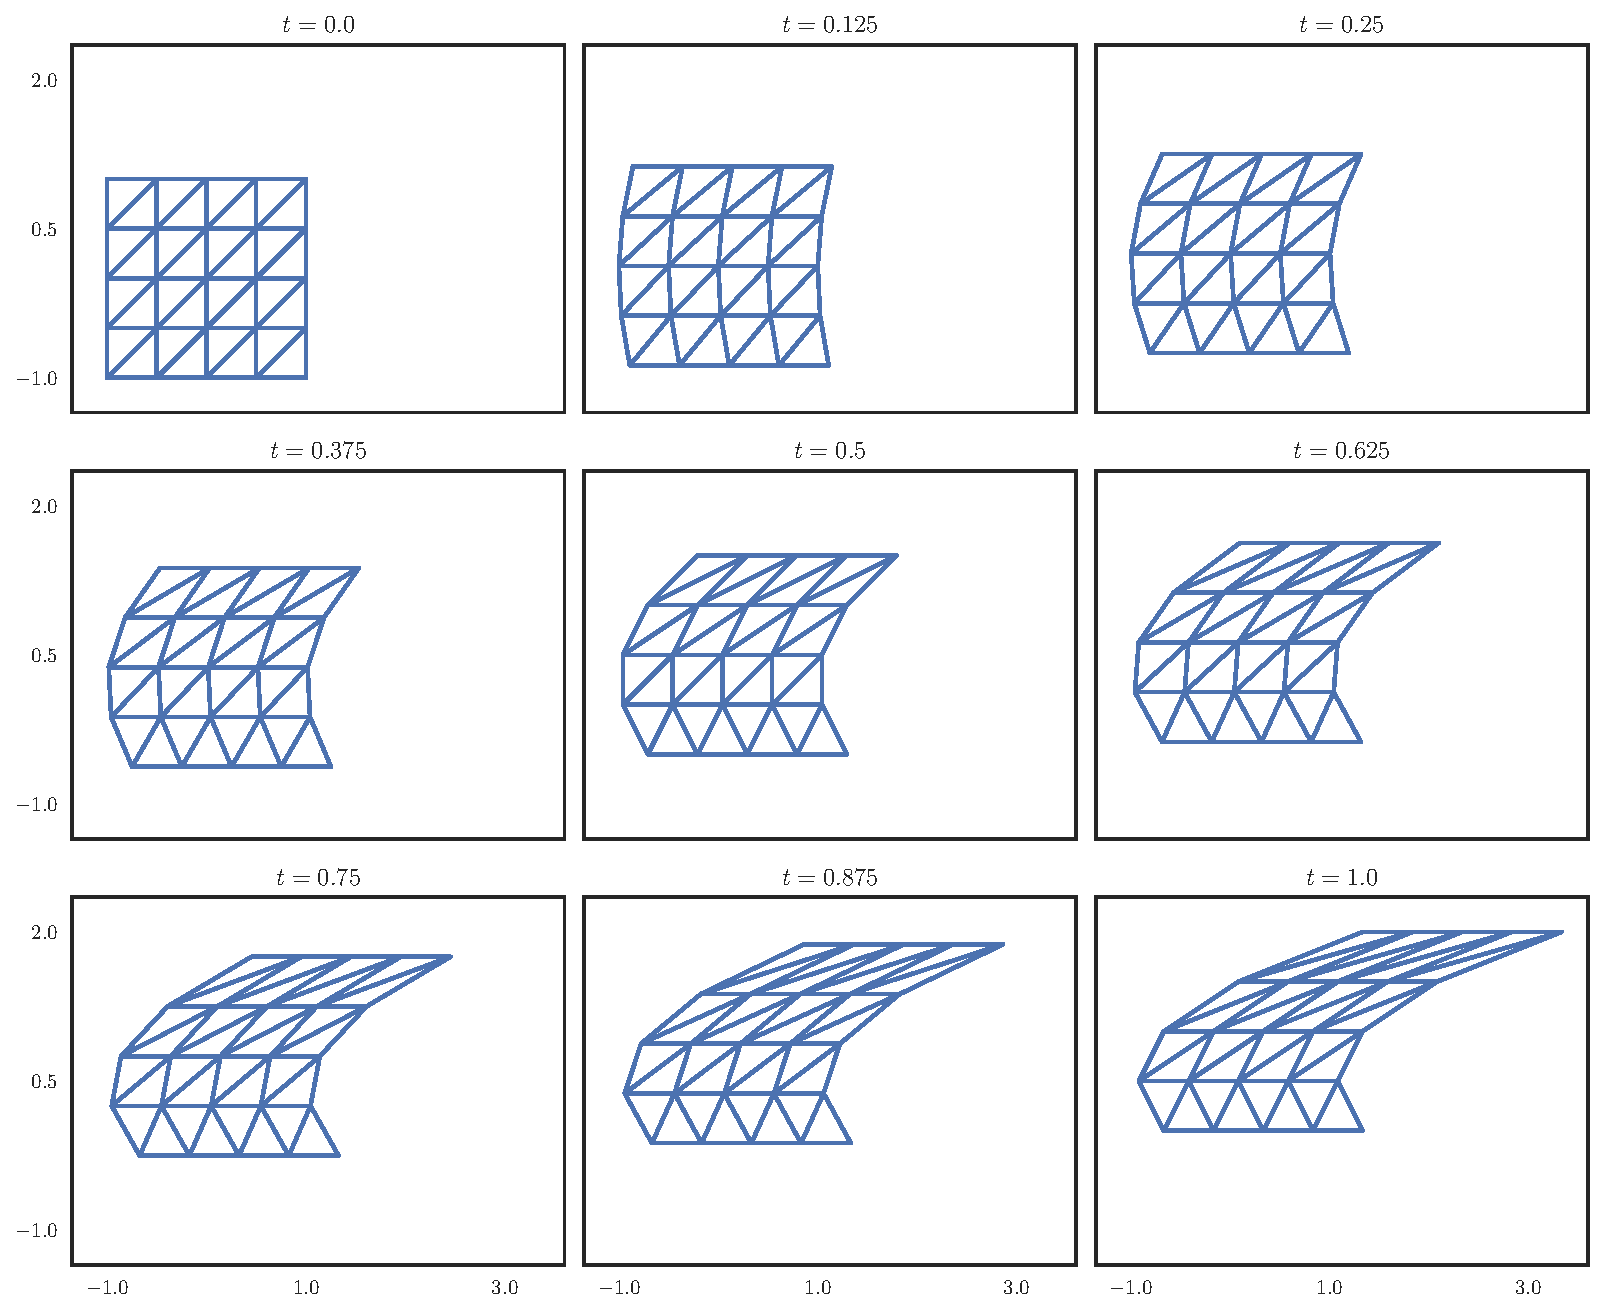
\includegraphics{../images/curved-mesh/mesh_distortion.pdf}
  \centering
  \captionsetup{width=.75\linewidth}
  \caption{Distortion of a regular mesh caused by particle motion along
    the velocity field \(\left[ y^2 \; 1 \right]^T\) from \(t = 0\)
    to \(t = 1\) with \(\Delta t = 1/4\).}
  \label{fig:mesh-distortion}
\end{figure}

A flow-based change to a mesh can cause problems if it causes the mesh to
leave the domain being analyzed or if it distorts the mesh until the element
quality is too low in some mesh elements. Over enough time, the mesh can
even tangle (i.e. elements begin to overlap).
For an example of such distortion (Figure~\ref{fig:mesh-distortion}),
consider a PDE of the form
\begin{equation}\label{eq:non-rigid-characteristics}
u_t + \left[ \begin{array}{c} y^2 \\ 1 \end{array}\right] \cdot \nabla u +
  F\left(u, \nabla u\right) = 0.
\end{equation}
The characteristics \(y(t) = y_0 + t, x(t) = x_0 +
\left(y(t)^3 - y_0^3\right)/3\)
distort the mesh considerably after just one second.

\begin{figure}
  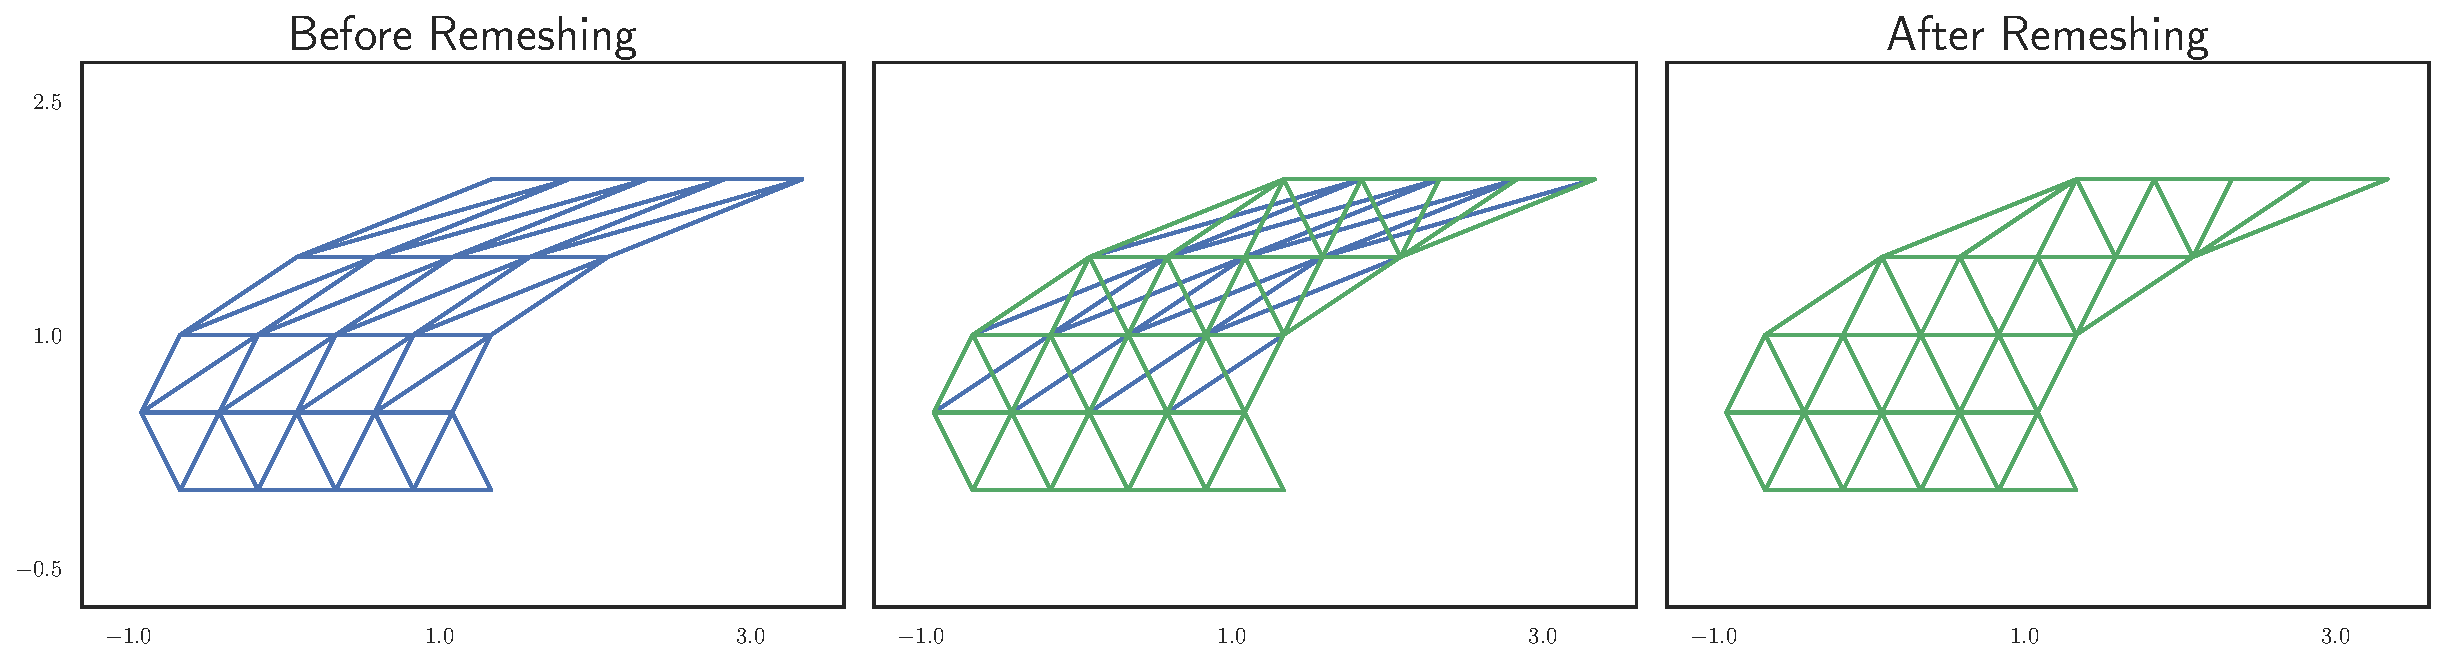
\includegraphics[width=0.9375\textwidth]
                  {../images/curved-mesh/distortion_remesh.pdf}
  \centering
  \captionsetup{width=.75\linewidth}
  \caption{Remeshing a domain after distortion caused by particle motion
    along the velocity field \(\left[ y^2 \; 1 \right]^T\) from \(t = 0\)
    to \(t = 1\).}
  \label{fig:distortion-remesh}
\end{figure}

To deal with distortion, one can allow the mesh to adapt in between time
steps. For example, Figure~\ref{fig:distortion-remesh} shows an example
remeshing of the domain.
In addition to improving mesh quality, mesh
adaptivity can be used to dynamically focus computational effort to resolve
sensitive features of a numerical solution. From~\cite{Iske2004}
\begin{quote}
{\small In order to balance the method's approximation quality and its
computational costs effectively, adaptivity is an essential requirement,
especially when modelling multiscale phenomena.}
\end{quote}
For more on mesh adaptivity,
see \cite{Dukowicz1987, Babuska1978, Iske2004}.

In either case, the change in the
mesh between time steps requires transferring a known solution on the
discarded mesh to the mesh produced by the remeshing process. Without
the ability to change the mesh, Lagrangian methods (or, more generally,
ALE~\cite{Hirt1974}) would not be useful, since after a limited time the
mesh will distort.

\subsection{High-order Meshes}

\begin{figure}
  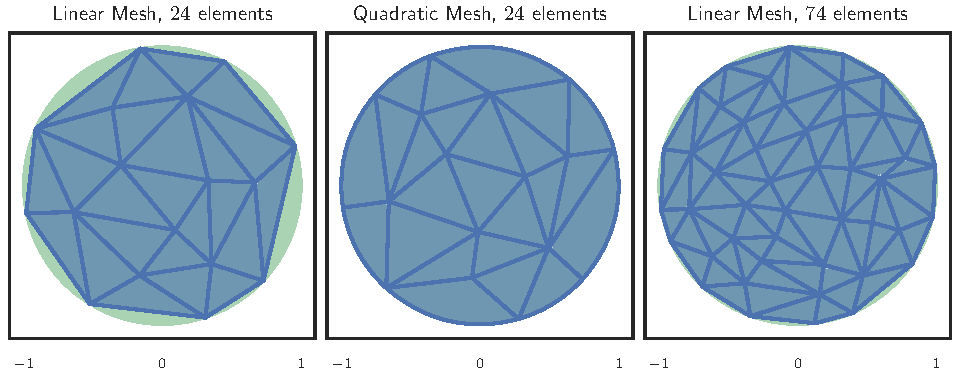
\includegraphics[width=0.9375\textwidth]
                  {../images/curved-mesh/main_figure27.pdf}
  \centering
  \captionsetup{width=.75\linewidth}
  \caption{Comparing straight sided meshes to a curved mesh when approximating
    the unit disc in \(\reals^2\).}
  \label{fig:curved-vs-straight-mesh}
\end{figure}

To allow for greater geometric flexibility and for high order of convergence,
curved mesh elements can be used in the finite element method. Though the
complexity of a method can steeply rise when allowing curved elements, the
trade for high-order convergence can be worth it. (See~\cite{Wang2013} for
more on high-order CFD methods.) Curved meshes can typically
represent a given geometry with far fewer elements than a straight sided mesh
(for example, Figure~\ref{fig:curved-vs-straight-mesh}).
The increase in accuracy also allows for the use of fewer elements, which
in turn can also facilitate a reduction in the overall computation time.

\begin{figure}
  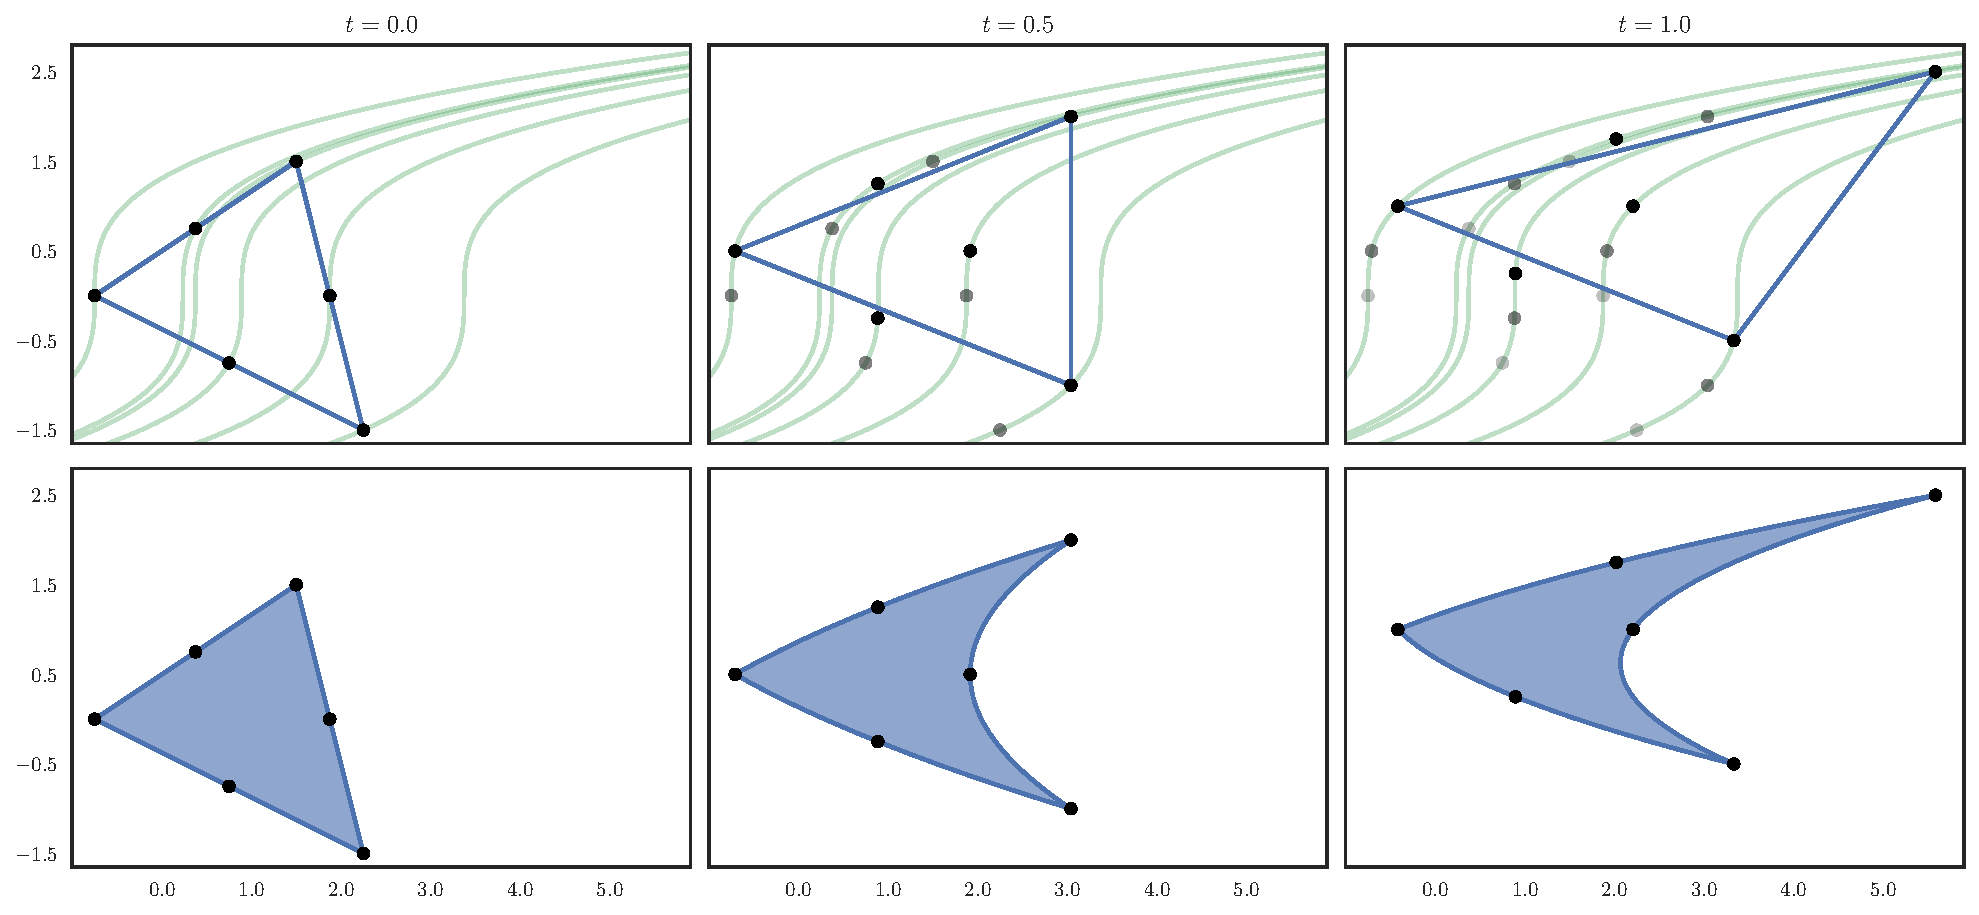
\includegraphics{../images/curved-mesh/element_distortion.pdf}
  \centering
  \captionsetup{width=.75\linewidth}
  \caption{Movement of nodes in a quadratic element under distortion caused
    by particle motion along the velocity field \(\left[ y^2 \; 1 \right]^T\)
    from \(t = 0\) to \(t = 1\) with \(\Delta t = 1/2\). The green curves
    represent the characteristics that each node travels along.}
  \label{fig:element-distortion}
\end{figure}

Even if the domain has no inherent curvature, high-order (degree \(p\)) shape
functions allow for order \(p + 1\) convergence, which is desirable in
it's own right. However, even in such cases, a Lagrangian method must either
curve the mesh or information about the flow of the geometry will be lost.
Figure~\ref{fig:element-distortion} shows what happens to a given
quadratic element as the nodes move along the
characteristics from~\eqref{eq:non-rigid-characteristics}.
This element uses the triangle vertices and edge
midpoints to determine the shape functions. However, as the nodes move
with the flow, the midpoints are no longer on the lines connecting
the vertex nodes. To allow the mesh to more accurately represent the
solution, the edges can instead curve so that the midpoint nodes remain
halfway between (i.e. half of the parameter space) the vertex nodes along
an edge.

%% However, the basis functions of the donor mesh
%% are (in general) discontinuous piecewise polynomials over any given
%% element of the target mesh, which are very difficult to integrate
%% by numerical quadrature schemes.

%% B\'{e}zier curves and triangles were selected for defining
%% mesh elements for two main reasons...
%% Secondly, B\'{e}zier curves and triangles have a
%% number of mathematical properties leading to elegant
%% algorithms.

%% Since adapting the mesh changes the domain for \(\bm{f}\), we
%% must project \(\bm{f}\) onto the new mesh domain. This is
%% accomplished by making local projections of \(\bm{f}\) whenever
%% local mesh modifications are made, and then computing
%% the local reinterpolation error. The choice of a
%% relevant error norm and projection is problem dependent,
%% but the computations are generally easy, since
%% they are done in a local setting with few degrees of
%% freedom. If the calculated re-interpolation error due
%% to a mesh modification is too great, then the modification
%% can be aborted and can be replaced with a mesh
%% refinement.

\subsection{Multiphysics and Comparing Methods}

In multiphysics simulations, a problem is partitioned into physical components.
This partitioning can apply to both the physical domain (e.g. separating a
solid and fluid at an interface) and the simulation data itself (e.g. solving
for pressure on one mesh and velocity on another). Each (multi-)physics
component is solved for on its own mesh. When the components interact, the
simulation data must be transferred between those meshes.

In a similar category of application, data transfer enables the comparison
of solutions defined on different meshes. For example, if a reference
solution is known on a very fine special-purpose mesh, the error can be
computed for a coarse mesh by transferring the solution from the fine
mesh and taking the difference. Or, if the same method is used on
different meshes of the same domain, the resulting computed solutions can
be compared via data transfer. Or, if two different methods use two
different meshes of the same domain.

\subsection{Limitations}

\begin{figure}
  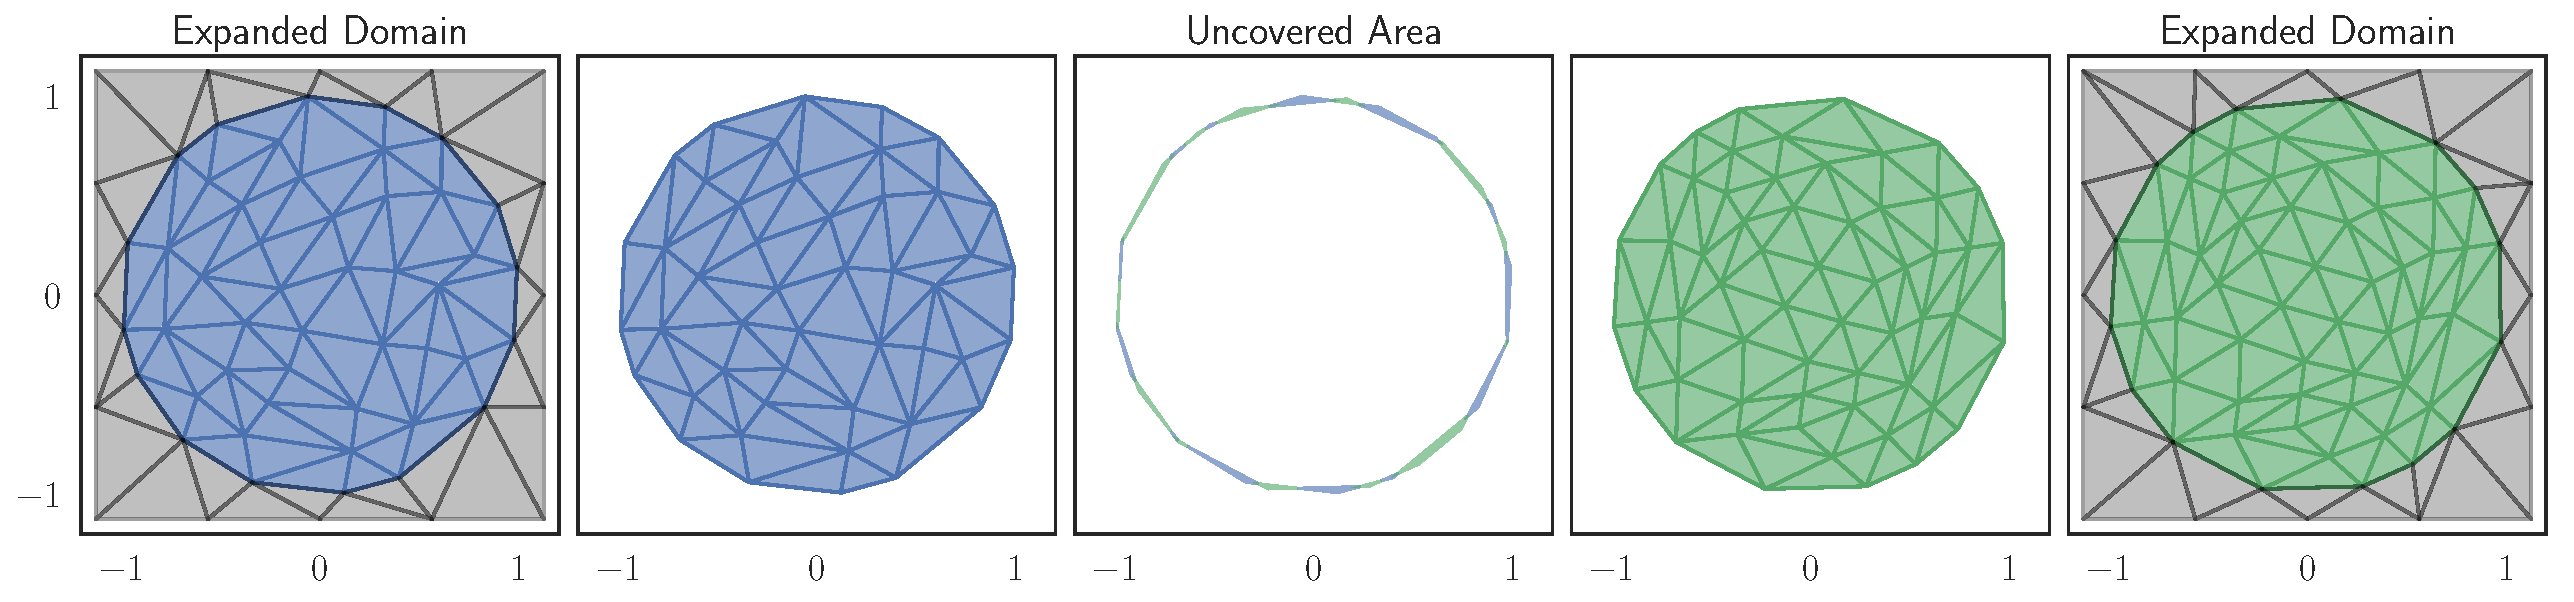
\includegraphics[width=0.96875\textwidth]
                  {../images/curved-mesh/main_figure29.pdf}
  \centering
  \captionsetup{width=.75\linewidth}
  \caption{Partially overlapping meshes on a near identical domain. Both are
    linear meshes that approximate the unit disc in \(\reals^2\). The outermost
    columns show how the domain of each mesh can be expanded so they agree.}
  \label{fig:partially-overlapping}
\end{figure}

The method described in this work only applies to meshes in \(\reals^2\).
Application to meshes in \(\reals^3\) is a direction for future research,
though the geometric kernels (see Chapter~\ref{chap:bezier-intersection})
become significantly more challenging to describe and implement. In
addition, the method will assume that every element in the
target mesh is contained in the source mesh. This ensures that the data
transfer is \textit{interpolation}. In the case where all target elements are
partially covered, \textit{extrapolation} could be used to extend a solution
outside the domain, but for totally uncovered elements there is no clear
correspondence to elements in the source mesh.

The case of partially overlapping meshes can be addressed in particular
cases (i.e. with more information). For example, consider a problem
defined on \(\Omega = \reals^2\) with no boundary condition and solution
that tends towards zero as points tend to infinity. A typical approach
may be to compute the solution on a circle of large enough radius and
consider the numerical solution to be zero outside the circle.
Figure~\ref{fig:partially-overlapping} shows how data transfer could be
performed in such cases when the meshes partially overlap: construct a
simple region containing both computational domains and then mesh the
newly introduced area. However, the assumption that the numerical solution
is zero in the newly introduced area is very specific and
a similar approach may not apply in other cases of partial overlap.

Some attempts (\cite{Berger1987, Chesshire1994, Cai1999}) have been
made to interpolate fluxes between overlapping meshes. These perform
an interpolation on the region common to both meshes and then numerically
solve the PDE to determine the values on the uncovered elements.

\section{Curved versus Polygonal Computing}

\begin{figure}
  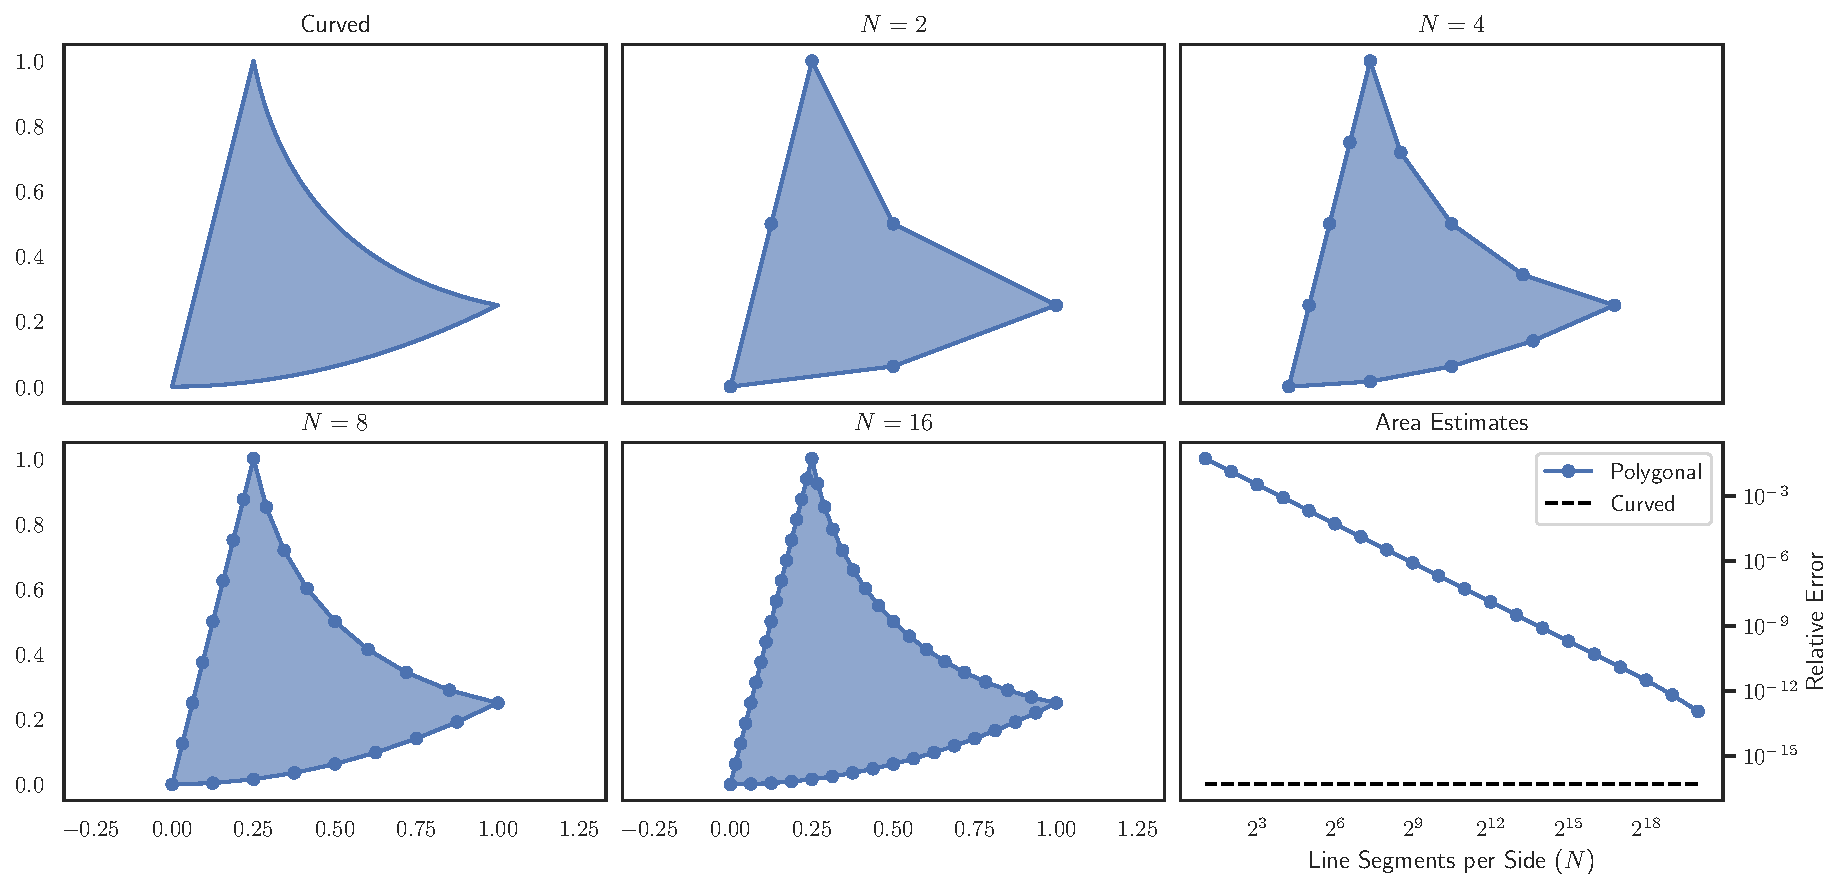
\includegraphics[width=0.9375\textwidth]
                  {../images/curved-mesh/polygon_vs_curved.pdf}
  \centering
  \captionsetup{width=.75\linewidth}
  \caption{Comparing the relative error for the computed area of a quadratic
    B\'{e}zier triangle. In one method, the curved boundary is used with
    Green's method and it is correct to machine precision. In the other,
    the curved edges are approximated by polygonal paths. These paths are
    generated from equally spaced parameters, for example a B\'{e}zier curve
    \(b(s)\) with \(N = 4\) would be approximated by a line connecting
    \(b(0), b(1/4), b(1/2), b(3/4)\) and \(b(1)\).}
  \label{fig:polygon-vs-curved}
\end{figure}

\begin{figure}
  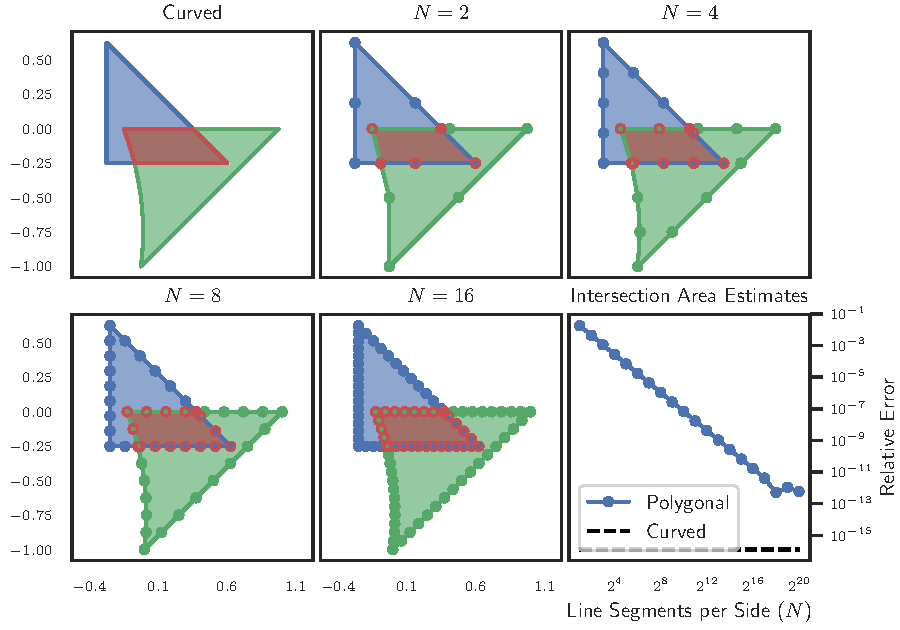
\includegraphics[width=0.9375\textwidth]
                  {../images/curved-mesh/polygon_vs_curved_intersection.pdf}
  \centering
  \captionsetup{width=.75\linewidth}
  \caption{Comparing the relative error for the computed area of the
    intersection of two quadratic B\'{e}zier triangles. In one method, the
    intersection boundary is fully specified as the union of B\'{e}zier curve
    segments and the area is found via Green's method. This method is correct
    to machine precision. In the other, the curved edges are approximated by
    polygonal paths and the intersection of the resulting polygons is computed.
    These paths are generated from equally spaced parameters, for example a
    B\'{e}zier curve \(b(s)\) with \(N = 4\) would be approximated by a line
    connecting \(b(0), b(1/4), b(1/2), b(3/4)\) and \(b(1)\).}
  \label{fig:polygon-vs-curved-intersection}
\end{figure}
